\documentclass{article}
\usepackage[spanish]{babel}   
\usepackage[numbers,sort&compress]{natbib}
\usepackage{float}
\usepackage{graphicx} 	% Nos permite importar imagenes 

\begin{titlepage}
	\begin{center}
	\line(1,0){300}\\
	[0.25in]
	\huge{\bfseries Reporte.- Tarea 1 }\\
	[2mm]
	\line(1,0){200}\\
	[1.5cm]
	\textsc{\LARGE Victor Alejandro Oviedo Martínez}\\
	[0.75cm]
	\textsc{\Large 15 de Septiembre del 2020\\}\\
	[10cm]
	\end{center}
	\begin{flushright}
	\textsc{\large Cd. Universitaria \\
	San Nicolás de los Garza, N.L. \\
	\# 66451\\}
	\end{flushright}
\end{titelpage}
\newpage

\begin{document}
\section{Introducciòn}\label{intro}


\newline

Para esta primera tarea se a estudiado el movimiento Browniano, en el cual nos habla acerca de la representación de una partícula la cual tiene la capacidad de realizar movimiento al azar con dirección y magnitud discretizados, tomando en cuenta que su posición inicial será el origen. Una vez estudiado las capacidades del movimiento Browniano se a podido ver simulaciones ejemplo con el fin de entender la tarea a realizar.

\section{Desarrollo}

Para esta primera tarea se a planteado el siguiente problema:
Examina de manera sistematica los efectos de la dimension en el tiempo de regreso al origen del movimiento Browniano para dimensiones 1 a 8 en incrementos lineales de uno, variando el numero de pasos de la caminata como potencias de dos con exponentes de 5 a 10 en incrementos lienales de uno, con 50 repeticiones del experimento para cada combinacion. Grafica los resultados en unsa sola figura con diagrama de caja de bigote o violin, colocando y coloreando los resultados de una distancia y otra de tal manera que es facil concluir si la distancia utilizada tiene algun efecto en el comportamiento, o en su defecto, incluir un cuadro indicando el minimo, proemdio maximo del tiempo de regreso por cada dimension junto con el porcentaje de caminatas que nunca regresaron.
\newline

El programa empieza importando librerías importantes, como la generación de números pseudo-aleatorios, la librería para graficar, y la librería para la función “inf”.   Después se inicializan variables para los contadores X y Y, luego tendremos la definición de las funciones las cuales empiezan con en contador X y Y siguiendo con la función paso y experimento.
\newline

contadorx(x,y) y contadory(y) .- Estas dos funciones ralamente funcionan en conjunto, ya que el propósito del contador X es contar del numero 5 hasta el 10, sin embargo, esta función no tiene la posibilidad de auto guardarse el valor para el reinicio, por lo tanto, se utiliza Y para recordar su posición.
\newline


paso(pos, dim).- esta función se encarga de elegir una dimensión, y una vez elegida una dimensión, se procede a elegir dirección para moverse en esta esta función te da de regreso el movimiento en una dimensión especifica.
\newline


experimento (largo, dim, tiempo, t, x, y).- Nos genera siempre un vector de posición en el origen, para después repetir la secuencia conjunta de contador(x,y), contador(y) y paso(pos,dim), esto con el fin de contar el tiempo que tarda la partícula en regresar al origen. De no regresar al origen en el tiempo máximo asignado a la caminata, se le asignará valor infinito.
\newline
\newline

A esto se le agrega la inicialización de algunas variables como; rep, largo, total, pasos, y regresos.
\newline


 Se podría decir que real mente el programa inicia con el ciclo “for i in rep:”, en donde este tiene la función de repetir el experimento para las 8 dimensiones necesarias, y que a su vez repetirá las funciones contadorx(x,y), contadory (y), y paso(pos, dim), con el fin de simular todos los experimentos.
\newline





Por último, todos los vectores de los diferentes experimentos se agrupan en una sola variable para poder ser graficados. Ahora se hará mención ha los detalles que se tuvieron con este programa y no se encontraron solución. Revisando el programa que la maestra dejo como ejemplo, se tiene que, para graficar todos los valores generados por el programa, estos valores son agregados a una sola variable, en la cual cada ves que se generan los datos para una sola dimensión se agregan, y dado que este proceso se repetirá hasta completar el total de dimensiones, es solo cuestión de variar el vector en el cual se guardaran nuestros datos para al final tener todos los valores en una sola variable y con esto poder graficar todo el contenido.  Este procedimiento se intento exactamente como la maestra lo realiza en su código, sin embargo, al momento de correr el programa nos genera un error en el cual nos dice que en la línea 91 la variable en la que queremos agregar los datos no tiene el rango necesario. Siendo que si son del mismo tamaño. He dejado el código utilizado comentado sobre el código de la tarea para que se pueda ver a lo que hago referencia. Sin embargo, he intentado con un rango mas amplio y sea tenido el siguiente resultado.

\begin{figure}[H]
\begin{center}
	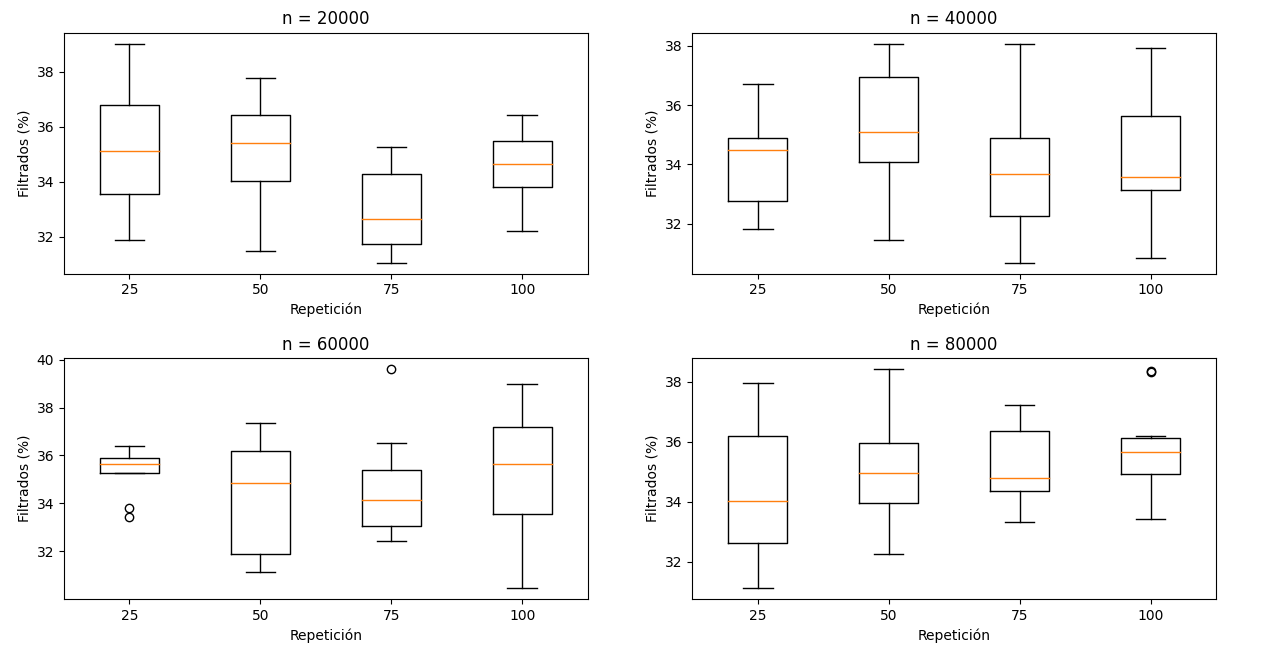
\includegraphics[height=3in]{/Users/victor/Desktop/Figure_2.png}
	\caption{Grafica con el error de rango}
	\label{fig:tarea.1}
\end{center}
\end{figure}


Como se puede observar en la Figura \ref{fig:tarea.1}, se pudo graficar los valores, sin embargó queda sin valores la dimensión 1. Por lo tanto, se guarda por así decirlo de forma manual los valores en la variable. Para después esta ser graficada. Por ultimo se logro graficar todos los valores de forma manual, pero correcta, sin embargó al código se le generan errores creo yo por el uso del valor “inf”, ya que en el proceso de conteo para el tiempo de regreso se a dejado un limite de pasos para este fin, de sobrepasarse este limite el programa esta programado para guardar el valor “inf” como resultado a ese experimento, por lo que imagino que al momento generarse la grafica, esta utiliza todos los valores guardados en el vector de datos y al tener valores infinitos se genera un error para el calculo de la misma.

\section{Conclusion}



Como concusión a los resultados de la Figura \ref{fig:tarea.2} y a la experiencia dejada por el desarrollo de esta tarea, se tiene que, para todas las dimensiones simuladas en este programa el tiempo de regreso mas frecuente se tiene en los primeros movimientos, ya que es mas probable avanzar un paso, y luego retrocederlo en la misma dimensión, que avanzar en diferentes y luego esperar que se genere el regreso en las mismas dimensiones. Aunado a la explicación anterior, se puede observar como mientras menos dimensiones se tengan mas aumenta el tiempo de regreso al origen. Por lo que con esto se reafirma nuestra suposición.

\begin{figure}[H]
\begin{center}
	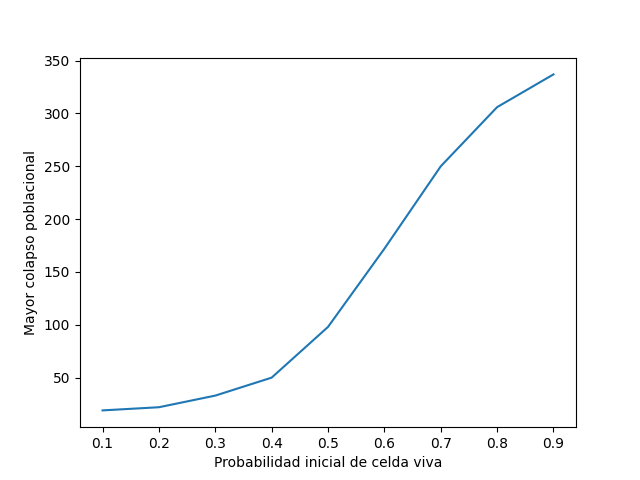
\includegraphics[height=3in]{/Users/victor/Desktop/Figure_1.png}
	\caption{Grafica Final}
	\label{fig:tarea.2}
\end{center}
\end{figure}

%\bibliography{ref.Tarea1.bib}
%\bibliographystyle{plainnat}

\end{document}
